\documentclass[10pt, a5paper]{article}
\usepackage{pdfpages}
\usepackage{parallel}
\usepackage[T2A]{fontenc}
\usepackage{ucs}
\usepackage[utf8x]{inputenc}
\usepackage[polish,english,russian]{babel}
\usepackage{hyperref}
\usepackage{rotating}
\usepackage[inner=2cm,top=1.8cm,outer=2cm,bottom=2.3cm,nohead]{geometry}
\usepackage{listings}
\usepackage{graphicx}
\usepackage{wrapfig}
\usepackage{longtable}
\usepackage{indentfirst}
\usepackage{array}
\newcolumntype{P}[1]{>{\raggedright\arraybackslash}p{#1}}
\frenchspacing
\usepackage{fixltx2e} %text sub- and superscripts
\usepackage{icomma} % коскі ў матэматычным рэжыме
\PreloadUnicodePage{4}

\newcommand{\longpage}{\enlargethispage{\baselineskip}}
\newcommand{\shortpage}{\enlargethispage{-\baselineskip}}

\def\switchlang#1{\expandafter\csname switchlang#1\endcsname}
\def\switchlangbe{
\let\saverefname=\refname%
\def\refname{Літаратура}%
\def\figurename{Іл.}%
}
\def\switchlangen{
\let\saverefname=\refname%
\def\refname{References}%
\def\figurename{Fig.}%
}
\def\switchlangru{
\let\saverefname=\refname%
\let\savefigurename=\figurename%
\def\refname{Литература}%
\def\figurename{Рис.}%
}

\hyphenation{admi-ni-stra-tive}
\hyphenation{ex-pe-ri-ence}
\hyphenation{fle-xi-bi-li-ty}
\hyphenation{Py-thon}
\hyphenation{ma-the-ma-ti-cal}
\hyphenation{re-ported}
\hyphenation{imp-le-menta-tions}
\hyphenation{pro-vides}
\hyphenation{en-gi-neering}
\hyphenation{com-pa-ti-bi-li-ty}
\hyphenation{im-pos-sible}
\hyphenation{desk-top}
\hyphenation{elec-tro-nic}
\hyphenation{com-pa-ny}
\hyphenation{de-ve-lop-ment}
\hyphenation{de-ve-loping}
\hyphenation{de-ve-lop}
\hyphenation{da-ta-ba-se}
\hyphenation{plat-forms}
\hyphenation{or-ga-ni-za-tion}
\hyphenation{pro-gramming}
\hyphenation{in-stru-ments}
\hyphenation{Li-nux}
\hyphenation{sour-ce}
\hyphenation{en-vi-ron-ment}
\hyphenation{Te-le-pathy}
\hyphenation{Li-nux-ov-ka}
\hyphenation{Open-BSD}
\hyphenation{Free-BSD}
\hyphenation{men-ti-on-ed}
\hyphenation{app-li-ca-tion}

\def\progref!#1!{\texttt{#1}}
\renewcommand{\arraystretch}{2} %Іначай формулы ў матрыцы зліпаюцца з лініямі
\usepackage{array}

\def\interview #1 (#2), #3, #4, #5\par{

\section[#1, #3, #4]{#1 -- #3, #4}
\def\qname{LVEE}
\def\aname{#1}
\def\q ##1\par{{\noindent \bf \qname: ##1 }\par}
\def\a{{\noindent \bf \aname: } \def\qname{L}\def\aname{#2}}
}

\def\interview* #1 (#2), #3, #4, #5\par{

\section*{#1\\{\small\rm #3, #4. #5}}

\def\qname{LVEE}
\def\aname{#1}
\def\q ##1\par{{\noindent \bf \qname: ##1 }\par}
\def\a{{\noindent \bf \aname: } \def\qname{L}\def\aname{#2}}
}


\begin{document}

\title{Применение Clojure в web-разработке}%\footnote{Текст данных и последующих тезисов, кроме специально оговоренных случаев, доступен под лицензией Creative Commons Attribution-ShareAlike 3.0}

\author{Дмитрий Бушенко\footnote{Минск, Беларусь; \url{nop@list.ru}}}
\maketitle

\begin{abstract}
Clojure is a modern dialect of Lisp intentionally designed for seamless integration with  JVM-platform. Due to its functional nature and Lisp flexibility, Clojure suits well for web-applications development. A lot of of libraries written in functional style make web-development with Clojure really simple.
\end{abstract}

В 2007 году был представлен язык программирования Clojure \cite{Bushenko1}, быстро завоевавший популярность в кругах любителей Lisp"=а и функциональнй парадигмы. Автор языка, Рич Хикки, был недоволен существовавшими на то время реализациями Lisp"=а в основном из"=за того, что они плохо интегрировались с существующими платформами. Кроме того, в диалектах Lisp"=а, стандартизированных несколько десятков лет назад, содержится много устаревших технологий и синтаксиса.

Язык Clojure создавался для того, чтобы преодолеть указанные недостатки. Clojure обладает более удобным и современным синтаксисом, максимально ориентирующим пользователя на функциональную парадигму. Несмотря на динамическую типизацию языка, программы на Clojure компилируются в jvm"=байткод и бесшовно интегрируются с существующими java"=программами. Сейчас Clojure реализован уже для нескольких платформ, наиболее заметные из которых: JVM, .NET и JavaScript.

Язык Clojure является также и выражением идей Рича Хикки о том, насколько простым должен быть инструмент разработчика. В Clojure обычно используются всего четыре структуры данных (список, вектор, отображение и множество), вокруг которых построен основной API. Основная абстракция языка Clojure "--- это чистая функция, не имеющая побочных эффектов и, таким образом, гораздо больше приспособленная для повторного использования.

На сегодняшний день для Clojure написано большое количество библиотек \cite{Bushenko2}, в том числе и для разработки веб"=приложений. Они пропитаны духом Clojure, философией простоты и модульности. В мире Clojure не приветствуются фреймворки, ведь конкурирующие фреймворки отвратительно сочетаются вместе в одном приложении. Программа на Clojure "--- это конструктор с открытой архитектурой, в которой никто не навязывает вам  выбор каких"=то библиотек только из"=за того, что вы прежде выбрали уже другие. Например, Java"=программисты с трудом связывают вместе Spring, Guice и JEE, если вообще берутся за такое. Но что если вам нравится какая"=то часть одного фреймворка, и какая"=то другого? Разве вам не хотелось бы использовать их оба вместе?

В Clojure для каждого архитектурного уровня есть множество альтернатив, среди которых вы можете выбрать одну или несколько библиотек сразу (рис. \ref{fig:Bushenko1}).

\begin{figure} [h]
  \centering
  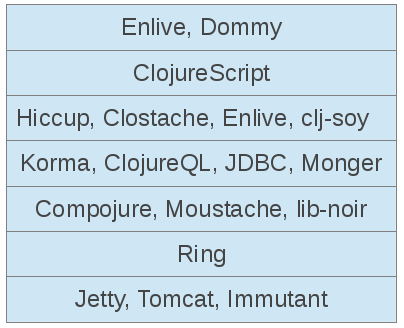
\includegraphics[height=4cm]{119_2013_w_figure1}
\caption{Библиотеки Сlojure для различных модулей архитектуры веб"=приложения}\label{fig:Bushenko1}
\end{figure}


\begin{figure}[h]
  \centering
  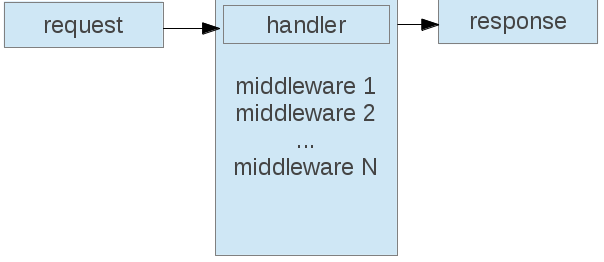
\includegraphics[height=3cm]{119_2013_w_figure2}
\caption{Ring}\label{fig:Bushenko2}
\end{figure}


Уровень маршрутизатора реализуют библиотеки Ring, \linebreak Compojure и Moustache.

Ring "--- это практически голый сервлет, каким он был бы, если бы его написали в функциональном стиле \cite{Bushenko3}. Центральная абстракция этой библиотеки "--- handler, который обрабатывает request и создает response (рис. \ref{fig:Bushenko2}). И request, и response "--- это обычные структуры данных Clojure "--- отображения. Композиция из функций"=middleware и handler"=ов задают бизнес"=логику обработки запроса. Как видите, это строгий функциональный подход.



Mustache и Compojure "--- это небольшие надстройки над Ring, каждый из которых по"=своему упрощает отображение маршрутов на функции, их обрабатывающие.

Уровень доступа к данным представлен несколькими интересными библиотеками, наиболее заметные из которых "--- это Korma и ClojureQL.
Korma "--- это библиотека, декларирующая, что она все"=таки не ORM \cite{Bushenko4}. Учитывая функциональную природу программ на Clojure, Object"=Relational Mapping"=у здесь и впрямь взяться неоткуда. Результаты запросов к БД представлены в виде векторов и отображений, а сами запросы записываются на удобном предметно"=ориентированном языке, внешне сильно напоминающем SQL.

ClojureQL схожа с Korma в том, что это предметно"=ориентированный язык \cite{Bushenko5}. Но, в отличие от Korma, семантика ClojureQL ближе к чистой реляционной алгебре, нежели к SQL.

Уровень представления реализуется целым рядом библиотек, соответствующих современным тенденциям. Hiccup "--- это то, как выглядел бы Haml, если бы его изначально написали на Clojure \cite{Bushenko6}. Clostache "--- это порт Mustache на Clojure, а clj"=soy "--- порт Google Closure Templates. Особенного внимания заслуживает библиотека Enlive, аналогов которой по сути и нету \cite{Bushenko7}. Она сильно напоминает XSLT т.к. занимается преобразованием исходного html"=файла по заданным правилам. Но, в отличие от XSLT, у которого громоздкий, неудобный синтаксис, Enlive делает все кратко и элегантно.
Важной частью инфраструктуры программ на Clojure является ClojureScript "--- реализация Clojure, компилирующегося в JavaScript \cite{Bushenko8}. Для ClojureScript также существует несколько шаблонизаторов, самые заметные из которых "--- Dommy \cite{Bushenko9} и Enfocus \cite{Bushenko10} (порт Hiccup и Enlive на ClojureScript). Использование Clojure на всех уровнях, начиная от доступа к БД, заканчивая UI"=логикой, позволяет отказаться от целого ряда лишних действий. Например, нет нужды генерировать ORM"=привязки к таблицам БД, очень упрощается передача данных с сервера на клиент, отпадает необходимость во всех промежуточных протоколах вроде SOAP или JSON.

Применение Clojure в web"=разработке позволяет также использовать всю гибкость Lisp"=а для построения предметно"=ориентированных языков. На примере библиотек доступа к данным мы видели, насколько удобно бывает разработать маленький, сфокусированный на определенном типе задач язык и решать задачи именно на нем. Clojure позволяет создавать такие языки с минимальными усилиями.

Таким образом, язык Clojure очень хорошо подходит для разработки web"=приложений. Он обладает отличной инфраструктурой, бесшовно интегрируется с любым java"=кодом и может деплоиться на стандартных серверах приложений java. Гибкость языка Clojure и его потрясающая выразительность позволяют создавать web"=приложения за минимальное время.

\begin{thebibliography}{99}

\bibitem{Bushenko1} Clojure, \url{http://clojure.org}
\bibitem{Bushenko2} Clojure Toolbox, \url{http://www.clojure-toolbox.com}
\bibitem{Bushenko3} Ring, \url{https://github.com/ring-clojure/ring}
\bibitem{Bushenko4} Korma, \url{http://sqlkorma.com}
\bibitem{Bushenko5} ClojureQL, \url{http://www.clojureql.org}
\bibitem{Bushenko6} Hiccup, \url{https://github.com/weavejester/hiccup}
\bibitem{Bushenko7} Enlive, \url{https://github.com/cgrand/enlive}
\bibitem{Bushenko8} ClojureScript, \url{https://github.com/clojure/clojurescript}
\bibitem{Bushenko9} Dommy, \url{https://github.com/Prismatic/dommy}
\bibitem{Bushenko10} Enfocus, \url{http://ckirkendall.github.com/enfocus-site}
\end{thebibliography}

\end{document}




